\documentclass[11pt,a4paper]{article}
\usepackage[margin=2.5cm]{geometry}
\usepackage{graphicx}
\usepackage{float}

\title{GALAH CNN Results}
\author{}
\date{}

\begin{document}

\maketitle

This document shows the result plots from the CNN model trained on the GALAH star spectra dataset. The model was used to predict the three labels $t\_eff$, $log\_g$, and $fe\_h$.

\section*{Result Plots}

\begin{figure}[H]
    \centering
    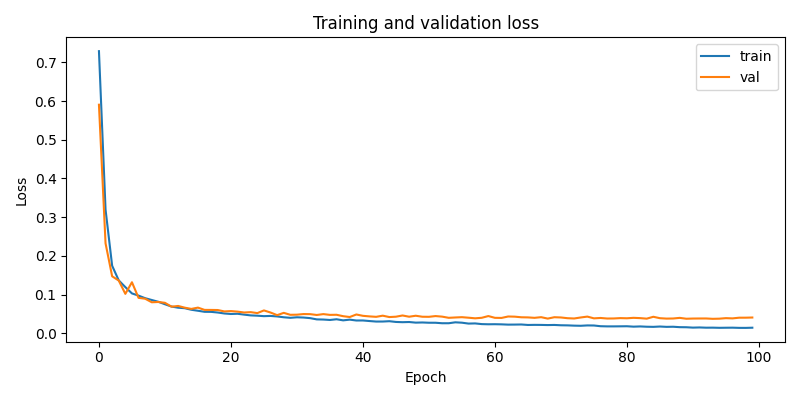
\includegraphics[width=0.75\linewidth]{../loss_curve.png}
    \caption{Loss curve.}
\end{figure}

\begin{figure}[H]
    \centering
    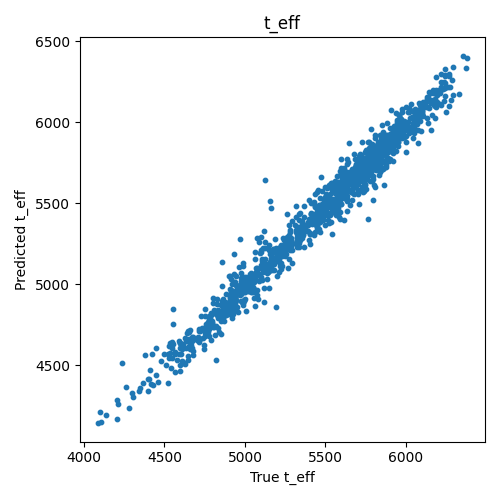
\includegraphics[width=0.75\linewidth]{../t_eff_pred_vs_true.png}
    \caption{$t_{eff}$ (effective temperature) prediction plot.}
\end{figure}

\begin{figure}[H]
    \centering
    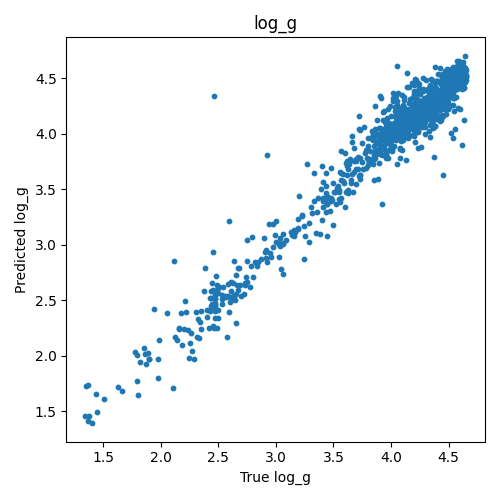
\includegraphics[width=0.75\linewidth]{../log_g_pred_vs_true.png}
    \caption{$log_g$ (surface gravity) prediction plot.}
\end{figure}

\begin{figure}[H]
    \centering
    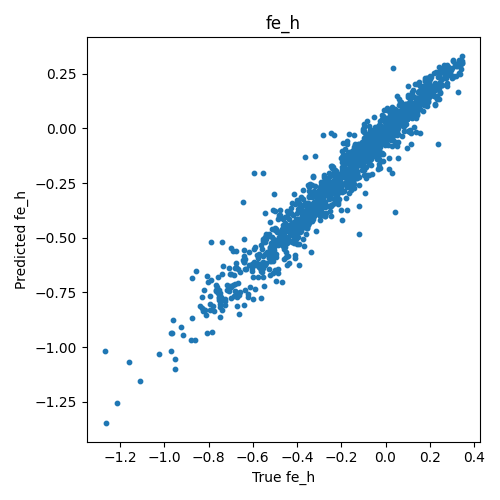
\includegraphics[width=0.75\linewidth]{../fe_h_pred_vs_true.png}
    \caption{$fe_h$ (metallicity) prediction plot.}
\end{figure}

\end{document}
